
%% NB: conversation with Helen Hanlon - suggested that 10 years overlap period is not really enough o be capture sufficient natural variability (problem not to do with sample size - so including more grid cells doesnt really help with this).
% One idea would be to do an additional comparison over a longer period between aggregated daily values form 2.2km model and CEH-GEAR Daily.

% \documentclass[APA,STIX2COL]{WileyNJDv5}
\documentclass[APA,Times2COL]{WileyNJDv5}
\usepackage{geometry}
\usepackage[parfill]{parskip}
\usepackage{tabularx}
\usepackage{booktabs}
\usepackage{lscape}
\usepackage{enumitem}
\usepackage{subcaption}
\usepackage[demo]{graphicx}
% \usepackage[table,xcdraw]{xcolor}
% \usepackage{amsmath}
% Include numbering for {paragraph|}
% \setcounter{secnumdepth}{4}
\usepackage{fontspec}
\usepackage{makecell}
\usepackage{todonotes}
\usepackage{afterpage}
\usepackage{tikz}
\usepackage{pgfplots}

\usepackage[export]{adjustbox}

\usepackage[utf8]{inputenc}
 
\usepackage[round]{natbib} % "round" will make the brackets like this: ()
\bibliographystyle{wileyNJD-APA.bst}
% \bibliographystyle{ajs.bst}

% \newcolumntype{C}[1]{>{\centering\arraybackslash}p{#1}}
\newcolumntype{L}[1]{>{\raggedright\let\newline\\\arraybackslash\hspace{0pt}}m{#1}}
\newcolumntype{C}[1]{>{\centering\let\newline\\\arraybackslash\hspace{0pt}}m{#1}}
\newcolumntype{R}[1]{>{\raggedleft\let\newline\\\arraybackslash\hspace{0pt}}m{#1}}

\newcommand{\subfigimg}[3][,]{%
  \setbox1=\hbox{\includegraphics[#1]{#3}}% Store image in box
  \leavevmode\rlap{\usebox1}% Print image
  \rlap{\hspace*{10pt}\raisebox{\dimexpr\ht1-2\baselineskip}{#2}}% Print label
  \phantom{\usebox1}% Insert appropriate spcing
}


% \setlength{\belowcaptionskip}{-10pt}
\graphicspath{{Figures/}} % Location of the graphics files

\title{\textbf{The sensitivity of urban surface water flooding to the temporal distribution of rainfall within events}}
\date{}
% \author{Molly Asher}

\geometry{verbose,tmargin=1cm,bmargin=3cm,lmargin=2cm,rmargin=2cm}

\begin{document}
\maketitle
\vspace{-1.5cm}
% \pagestyle{empty}
\pagenumbering{arabic}

\section{Abstract}

\todo[inline]{I know we talked about rephrasing the bit about testing the sensitivity of urban flood models to instead reference the sensitivity of urban flood modelling. I've done this, but not sure if the abstract now makes sense as a whole, and feel there is maybe still a bit of a lack of clarity about the focus on modelling methods vs. physical processes }

The risk posed globally by surface water flooding to people and properties is growing due to rapid urbanisation, infrastructure development and intensification of rainfall due to climate change. Surface water flooding generally occurs in the summertime, by rainfall from intense, localised convective storms. Whilst tools to model urban flood risk have also been rapidly developing, there remains a knowledge gap around the sensitivity of urban surface water flooding to the temporal distribution of rainfall within extreme convective storm events. In the UK, the industry standard flood modelling approach considers rainfall events to always be symmetrical, and with a singular peak in intensity. Extensive study of UK extreme rainfall observations suggests that loading of rainfall towards the start or end of events is in fact more common. In the present study, the sensitivity of flooding in two urban catchments in the north of England are tested using fifteen realistic rainfall profiles derived from observed extremes. These realistic events are compared to idealised profiles, constructed through making systematic variations to the industry standard profile to shift the single peak towards the start or end of the event. We demonstrate that the positioning of the peak, as well as its magnitude, influences the severity, timing and nature of the associated flooding. For events with the same rainfall volume, both catchments show approximately a 15\% increase in flooded area with the most back-loaded idealised profile compared to the most front-loaded, and a roughly 25\% increase with the most back-loaded observed profile compared to the most front-loaded. 

% The risk posed globally by surface water flooding to people and properties is growing due to rapid urbanisation, infrastructure development and intensification of rainfall. Whilst tools to model urban flood risk have also been rapidly developing, there remains a knowledge gap around the sensitivity of urban hydraulic modelling methods to the temporal structure of rainfall. In the UK, the industry standard process considers rainfall events to always be symmetrical, and with a singular peak in intensity. Extensive study of UK extreme rainfall events suggests that loading of rainfall towards the start or end of events is in fact more common. In the present study, the sensitivity of two urban catchments in the north of England are tested using profiles derived from making systematic variations to the industry standard profile to shift the single peak towards the start or end of the event. We demonstrate that the positioning of the peak, as well as its magnitude, influences the severity, timing and nature of the associated flooding. 

% In both catchments, for events with the same volume of rainfall, the most back-loaded profile results in approximately a 15\% increase in flooded area compared with the most front-loaded profile. We also consider fifteen realistic profiles derived from observed extremes. These profiles have diverse temporal patterns and also include significant variation in the magnitude of the peak intensity. In both catchments, for events with the same volume of rainfall, the most back-loaded profile results in approximately a 25\% increase in flooded area compared with the most front-loaded profile.

% In both catchments, for events with the same volume of rainfall, the most back load

% The risk posed globally by surface water flooding to people and properties is growing due to rapid urbanisation, infrastructure development and intensification of rainfall. Whilst tools to model urban flood risk have also been rapidly developing, there remains a knowledge gap around the sensitivity of urban landscapes to the temporal structure of rainfall. 

% In the UK, the industry standard flood hazard modelling approach considers rainfall events to always be symmetrical, and with a singular peak in intensity. Extensive study of UK extreme rainfall events suggests that loading of rainfall towards the start or end of events is in fact more common. In the present study, the sensitivity of two urban catchments in the north of England are tested using rain-on-grid hydraulic modelling. Idealised profiles are derived through making systematic variations to the industry standard profile to shift the single peak towards the start or end of the event. This allows us to demonstrate clearly and consistently that as the peak timing shifts towards the end of the event, the modelled flood becomes more extensive and severe.  Additionally, fifteen realistic profiles derived from the observed extremes are considered. This illustrates the the positioning of the peak, as well as its magnitude,

% This paper aims to build on this finding and to provide evidence on the extent to which hydrological response in a UK catchment shows sensitivity to this misrepresentation of storm temporal profil

% influences the severity, timing and nature of the associated flooding. 

% The profile with the latest peak results in an 18\% larger flooded area than the early peaking profile causing the smallest flooded area.

\section{Introduction}\label{sec:introduction}

Flooding is now the most frequently occurring and harmful natural hazard globally \citep{jenkins2018probabilistic, razavi2020anthropocene}. In the UK, roughly one-third of this overall flood risk is associated with surface water flooding \citep{houston2011pluvial}. Surface water flooding occurs when the volume of rainfall exceeds the absorption capacity of the ground and the storm water drainage capacity \citep{archer_characterising_2015}. It generally occurs in urban settings which tend to have a higher proportion of impermeable surfaces which preclude the natural processes that moderate floods in rural environments, causing a disproportionate amount of property damage. The rapid development of flooding during or after rainfall means that
surface water flooding is more more directly dependent on the rainfall characteristics within an event than fluvial flooding \citep{ochoa2015impact} (checkr ef no sentence has changed). 
% Understanding and accurately representing these dynamics is of paramount importance for accurate surface water flood risk modelling.

Flood modelling, like all forms of modelling, necessitates the use of simplifications to make complex natural phenomena manageable and comprehensible within computational frameworks. This simplification process involves making certain assumptions and approximations to represent the real-world processes that govern flooding. One notable simplification concerns the representation of rainfall \citep{bardossy2022precipitation}. Rainfall in flood models is commonly represented using design storms which are idealised rainfall events with simplified characteristics \citep{butler_urban_2004}. Design storms are advantageous as they avoid the need to model multiple individual historical rainfall events in a particular catchment and allow a standardised approach to assessing the impact of extreme rainfall \citep{balbastre2019comparison, marsalek1984design}. The total event rainfall depth is calculated through statistical analyses of historical rainfall data, and is generated for different durations and return periods. This depth is then distributed over time using a hyetograph which represents the time varying distribution of rainfall during a storm. The way in which the shape of the hyetograph is specified, and the impact of this on the resulting flood risk, is the focus of this work.

In the UK, the Flood Studies Report (FSR) and its successor, the Flood Estimation Handbook (FEH), have established a robust and widely accepted approach to flood modelling since the FSR was first published in 1975. Following this, the industry standard approach to flood risk modelling advises use of one of two design hyetographs specified in the FSR (note that whilst these profiles were initially derived in the FSR, they are now part of the contemporary FEH methods, and so from here forwards we refer to them as the FEH hyetographs). The FEH hyetographs are both symmetrical with a central peak in intensity. They are to be applied irregardless of the event duration or return period; with a summer profile, which is more sharply peaked, advised for use in urban areas, and a winter profile, which has a more shallow peak, recommended for rural catchments \citep{faulkner1999}. 

% In the UK, the Flood Studies Report (FSR) and its successor, the Flood Estimation Handbook (FEH), have established a robust and widely accepted approach to flood modelling since the FSR was first published in 1975. Following this, the industry standard approach to flood risk modelling advises use of one of two design hyetographs specified in the FSR (note that whilst these profiles were initially derived in the FSR, they are now part of the contemporary FEH methods, and so from here forwards we refer to them as the FEH hyetographs). The FEH hyetographs are both symmetrical with a central peak in intensity. They are to be applied irregardless of the event duration or return period; with a summer profile, which is more sharply peaked, advised for use in urban areas, and a winter profile, which has a more shallow peak, recommended for rural catchments \citep{faulkner1999}. 

There are a number of different approaches to specifying hyetographs. These are outlined in detail by \citet{chow1988applied}, \citet{veneziano1999best}, and \citet{balbastre2019comparison}, amongst others. The approaches can be loosely categorised as: observed (directly using temporal distributions from observed events); summary (generalising temporal distributions from observed events); stochastic (utilising stochastic rainfall models); or IDF curve-based methods (using rainfall characteristics from IDF (intensity duration frequency) curves alongside simple distribution shapes). The FEH profiles are best described as summary hyetographs, and were derived by study and generalisation of just 80 summer (May to October) and 32 winter (November to April) storms of 24-hour duration occurring between 1961 and 1970. The generalisation process is described in detail by Villalobos-Herrera (in press?). Importantly, in addition to the stages typical of generating summary hyetographs, an extra procedure is carried out which involves shifting each observed event's peak intensity to the centre. This ensures that when summary profiles are derived from averaging across multiple observed rainstorms, there is always a temporally central peak in intensity. Whilst much of the flood estimation methods associated with the FEH have been updated since the FSR's original release, the hyetographs have not been revised in the last fifty years. 

% Old evidence, and process that obfuscates temporal variability

Recent research indicates that the FEH hyetographs are not representative of the true variety in the timing of peak intensity in observed storms. A set of $\sim$70,000 UK independent rainstorms ranging from sub-hourly to daily durations were identified by \citet{herrera2023creation} using a new storm identification algorithm. These storms were used to trial an alternative approach to deriving summary hyetographs which removes the centering step applied in the FEH methodology. Rather, the positioning of the peak is made fundamentel to the hyetograph classification, with profiles classed as front-loaded, centred or back-loaded. Importantly, Villalobos-Herrera et al. (?) identify using this method that just 23\% of the observed storms have a central peak in intensity. This provides evidence that the majority of UK extreme storms are fundamentally different to design storms produced with the FEH hyetographs, and calls into question the validity of their continued application in UK flood modelling approaches. 

% This provides evidence that the majority of UK extreme storms are fundamentally different to design storms produced with the FSR hyetographs. This paper aims to build on this finding and to provide evidence on the extent to which this misrepresentation translates into significant differences in the flooding outcomes 

% this fundamental misrepresentation of storm temporal profiles translates into a significant difference in flooding outcome. 

This paper builds on the work of Villalobos-Herrera et al () to provide evidence on the extent to which hydrological response in a UK catchment shows sensitivity to this representation of storm temporal profile. The sensitivity of hydrological response to the temporal structure of rainfall is already evidenced in multiple studies. The majority of these studies focus on the impact of temporal profiles on flood peak discharge (\citet{fatone2021advanced}, \citet{dullo2017evaluation}, \citet{maca2009influence}, \citet{fadhel2018sensitivity}, \citet{wasko2015steeper}), in some cases with concurrent analysis of changes to the flood volume (\citet{lambourne1987model}, \citet{nguyen2010optimal}, \citet{peyron2002optimal}) or the time to peak (\citet{balbastre2019comparison}, \citet{ball1992influence}). Other studies have focused on flood depth alone \citep{hettiarachchi2018increase}, or more specific indicators, including the manhole overflow inundation area \citep{li2021case}, drainage system performance factors \citep{ng2020design}, and the capacity required in a storm water reservoir  \citep{pochwat2017temporal}. 

This existing research on storm temporal profiles and their impact on flooding outcomes leaves two notable gaps. First, while studies applying idealised profiles have tested a variety of simple, summary temporal patterns, they have often failed to conduct systematic adjustments to these profiles to assess the consequences of shifting the timing of the peak intensity. Second, there is an absence of research examining realistic observed rainfall profiles within the context of the UK. These two gaps underscore the need for further investigations to comprehensively analyse how variations in peak timing, both in idealised and real-world scenarios, influence flood risk assessments in urban catchments. The recent evidence provided by Villallobos-Herrera et al (in press) on the range of observed profiles within UK extremes, presents an opportunity to address these gaps. 

Specifically, the aims of this paper are to use rain-on-grid flood modelling to test the sensitivity of flood extent, depth and timing in an urban catchment to:

\begin{enumerate}
  \item The timing of the peak intensity in an idealised, single-peaked design storm 
  \item The range of temporal distributions in physically realistic hyetographs, and to quantify how these outcomes differ from using a single-peaked design storm 
\end{enumerate}

\begin{figure*}[htbp!]
\centering
\begin{subfigure}[b]{.65\textwidth}
\includegraphics[width=\linewidth]{Figs/Catchment/new_inset.png}\llap{
  \parbox[b]{4.3in}{(\textbf{a})\\\rule{0ex}{3.45in}}}\llap{
  \parbox[b]{1.5in}{(\textbf{b})\\\rule{0ex}{3.45in}}}
\end{subfigure}\qquad
\begin{subfigure}[b]{.3\textwidth}
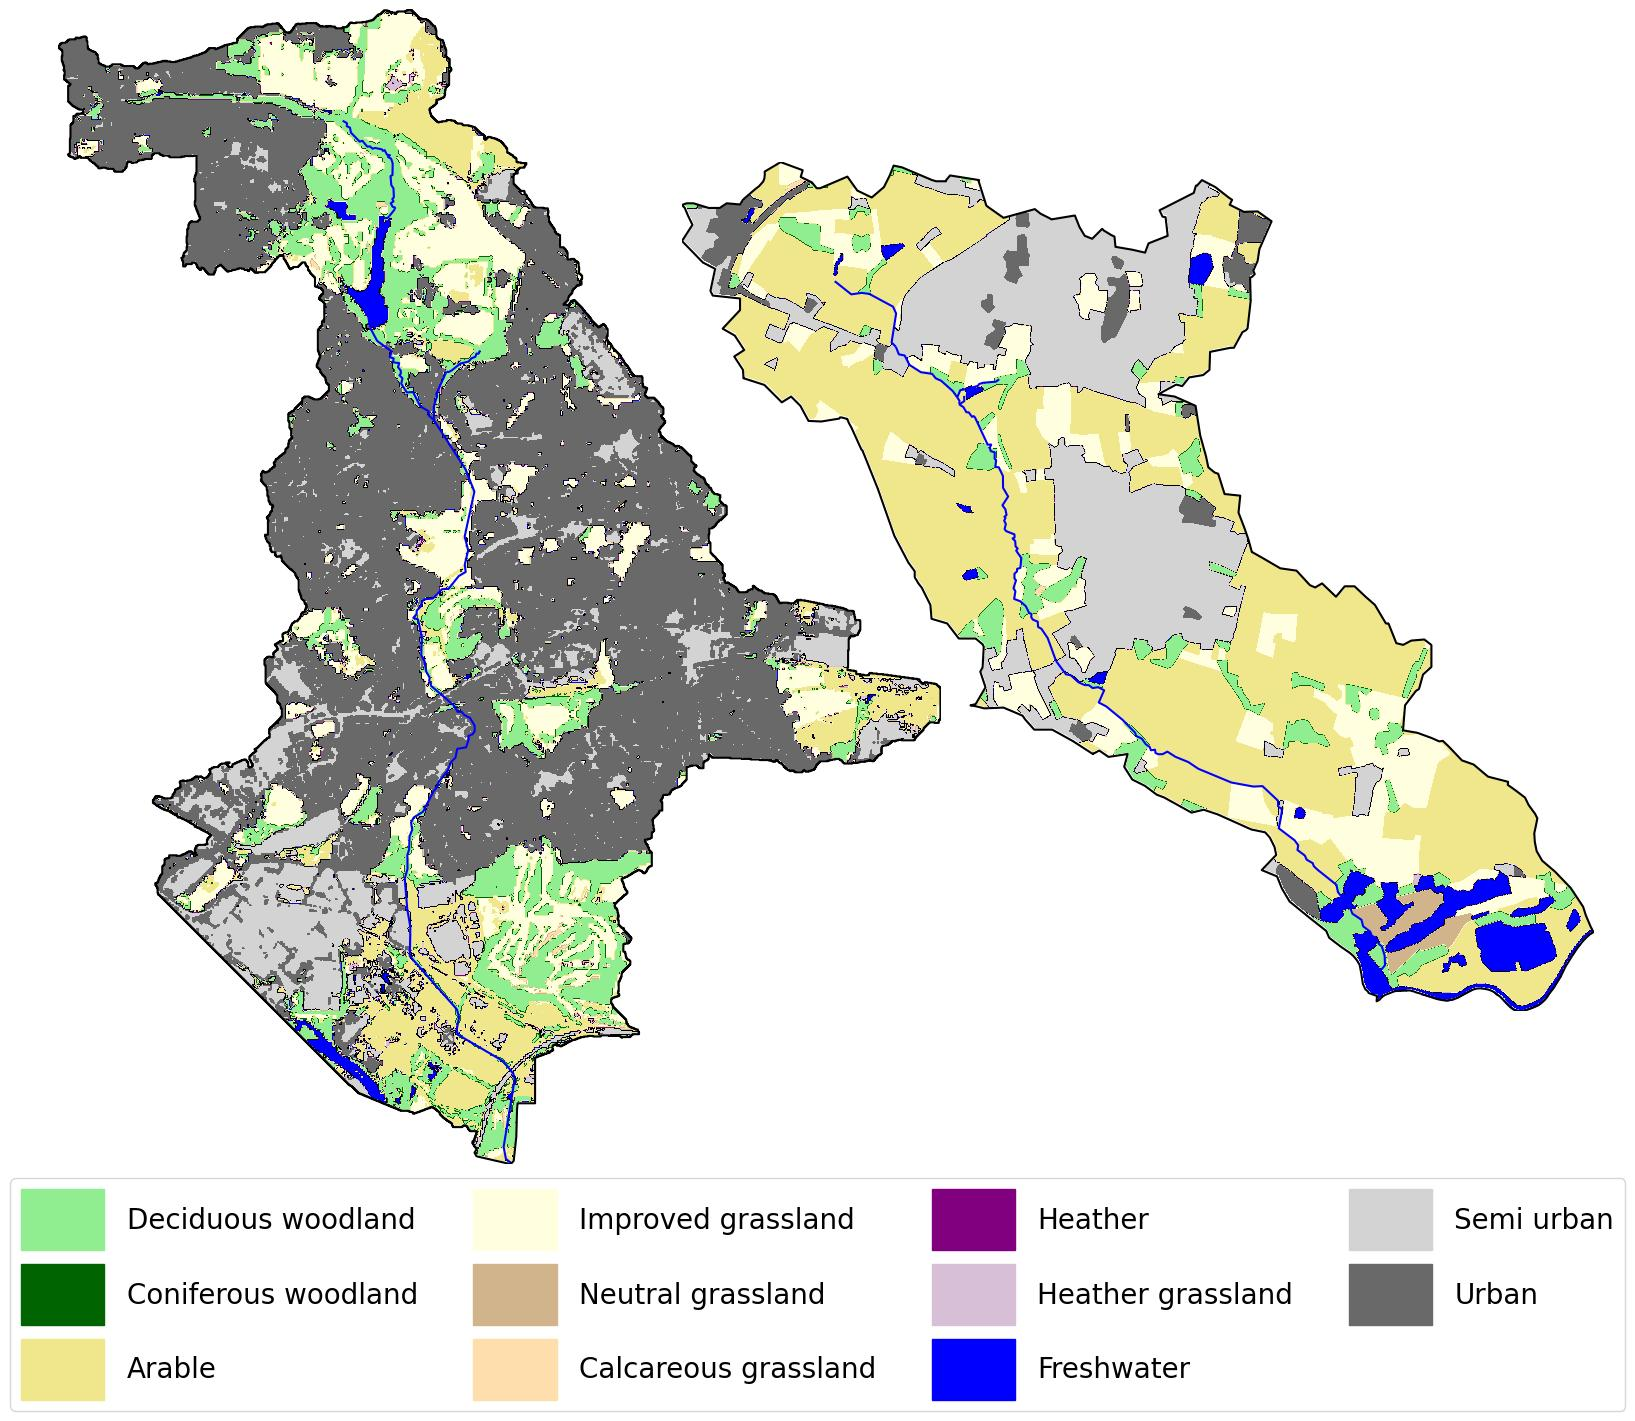
\includegraphics[width=0.99\textwidth]{Figs/Catchment/LandCover_BothCatchments.jpg}\llap{
  \parbox[b]{2.2in}{(\textbf{c})\\\rule{0ex}{1.6in}}}
% \vspace{2ex}
  \newline
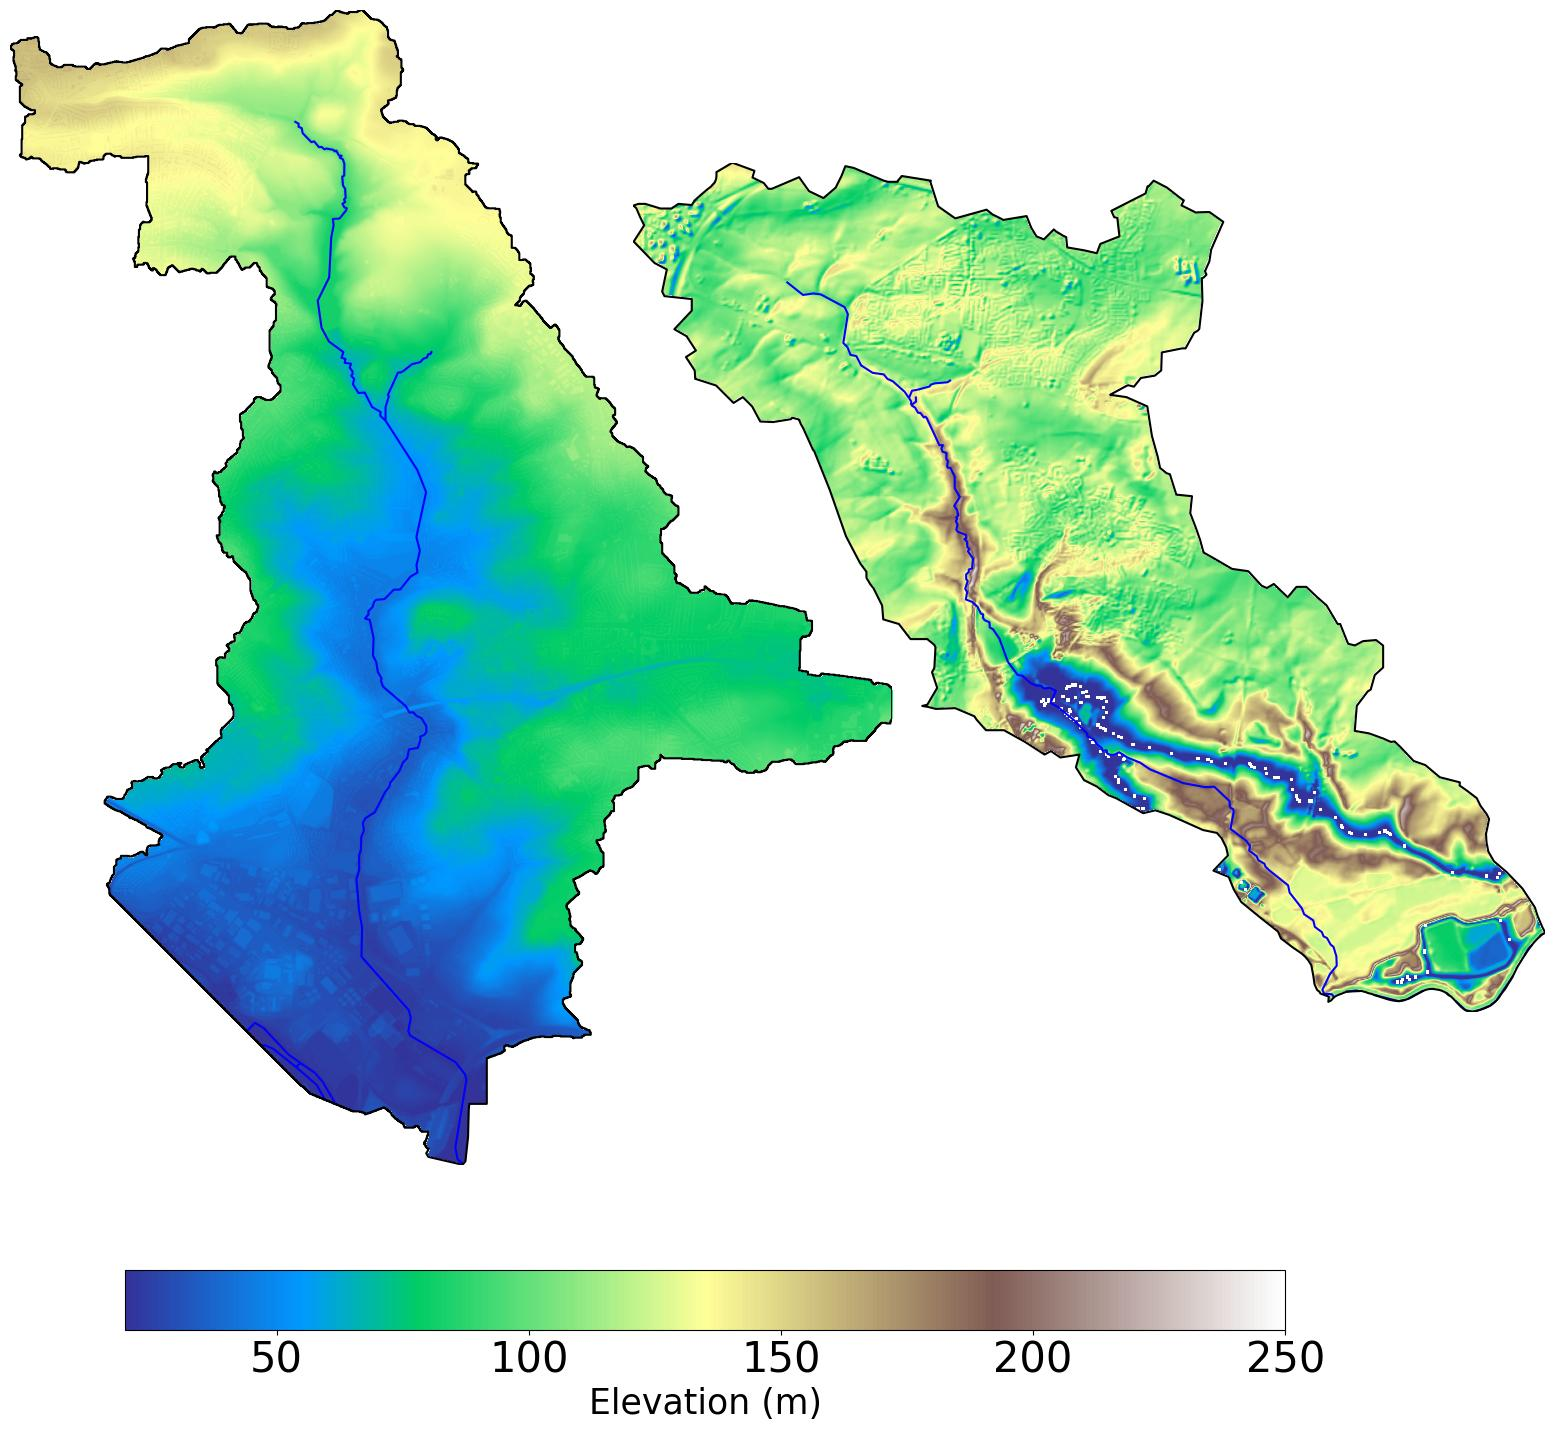
\includegraphics[width=0.99\textwidth]{Figs/Catchment/Terrain_BothCatchments.jpg}\llap{
  \parbox[b]{2.2in}{(\textbf{d})\\\rule{0ex}{1.5in}}}
\end{subfigure}
\caption{Geographical details of Wyke Beck (left) and Lin Dyke (right) catchments, (a) location in the wider Leeds area with the main watercourse marked (b) location in the UK, (c) land use and (d) topography} \label{fig:catchments}
\end{figure*}


\section{Methods}\label{sec:methods}
\subsection{The study catchments}\label{subsec:model:catchments}
Wyke Beck and Lin Dyke are two suburban catchments on the eastern edge of Leeds (Figure \ref{fig:catchments}a), in the north of England (Figure \ref{fig:catchments}b). Wyke Beck covers 33.6 km\textsuperscript{2}, and has a large (63\%) urban share, including numerous populous Leeds suburbs. It also includes a smaller proportion (36\%) of green spaces, such as woodland and parks, and a small (1\%) contribution from the permanent water in Waterloo Lake, to the north of the catchment, and Wyke Beck, a tributary of the river Aire (Figure \ref{fig:catchments}c). Lin Dyke covers 22.9 km\textsuperscript{2}, the majority (69\%) of the catchment is rural land uses, such as farmland and woodland, with a smaller proportion (27\%) made up of urban and suburban land uses around the settlements of Kippax and Garforth. The remainder of the catchment (4\%) is permanent water, which is primarily found in the wetlands in the downstream area of the catchment, which drain into the river Aire (Figure \ref{fig:catchments}c). Both catchments \texit{(comment on elevation -are these relatively high catchments? Or with particularly high variation?)} (Figure \ref{fig:catchments}d). 

\subsection{The flood inundation model}\label{subsec:model:catchments}

A 2D hydraulic rain-on-grid model is run in Hec-Ras 6.4.1 using the 2D unsteady diffusion wave equation set. Rain-on-grid modelling applies a rainfall input to each grid cell and simulates the movement of this water overland. Topography is defined with a Digital Elevation Model (DEM) and determines flow pathways and water ponding locations. Rain-on-grid modelling is a widely accepted approach to modelling surface water flood risk and was applied in the production of the Risk of Flooding From Surface Water (RoFSW) map \citep{environment2019risk}. There are some limitations to rain-on-grid modelling relating to the simplification or neglection of hydrological processes. The impact of these on our ability to assess the impact of the temporal profile on flood risk are discussed in Section \ref{sec:discussion}.
% maybe add a sentence about more specifically that we aren't reying to improve the modelling process but that it has implications for our understanding of the rainfall processes

Existing flood models are used for both Lin Dyke \citep{beadle2021} and Wyke Beck \citep{singh2023drainage} catchments. The land use data for Lin Dyke is the UK CEH 2019 Land Cover Map \citep{morton2020land} and for Wyke Beck (?). Both models use a `bare earth' LiDAR DEM, at a resolution of 1m for Lin Dyke and 2m for Wyke Beck (Environment Agency, 2020). The DEM is modified to ensure the watercourse is not obstructed completely at hydraulic structures, and to `stamp' on buildings to the terrain to ensure their impact on the flow is accounted for (Houston et al, 2011). 

The model is run for a total of 70 hours to ensure that the hydrological processes happening in the catchment after the storm are adequately captured. 
The model utilizes a variable time step, automatically adjusting it to maintain a Courant value within the range of 0.75 to 2. This adherence to the Courant condition ensures the stability of the simulation, with reliable and accurate results associated with a Courant value as close to 1 as possible.

% Limitations include the assumptions made in the data such as, no losses due to urban drainage, the variation in hydraulic roughness, and the resolution of the DTM.

\subsection{The rainfall data}\label{sec:rainfalldata}
Surface water flooding is associated with short duration, convective rainfall events \citep{rudd2020investigating}. A six hour duration was chosen for this study as \citep{beadle2021} suggested that in Lin Dyke this was the critical duration - the duration of rainfall event causing the highest peak flows (Davies & Hancock, 2015). This allows for a period of lighter rainfall either side of a peak (?). We modelled a 1-in-100 year return period event, considering it (as the middle of three options modelled in the Risk of Flooding from Surface Water map (Environment Agency, 2019)) a representative example of a moderately extreme scenario. The FEH web service provides rainfall depths associated with specific durations and return periods for UK catchments. This allowed us to define a rainfall depth of 59.29mm for Lin Dyke and 59.25mm for Wyke Beck.

% According to Megan's report REFH suggested 11 hours would be critical duration

Design storm profiles are required to translate this rainfall depth into the hyetographs which form the rainfall input to the flood model. We produce a hyetograph for each catchment using the FEH standard summer profile (e.g. black line, Figure \ref{fig:profiles}a), in order to establish a baseline - or standard - assessment of flood risk in the catchments. This is generated using the Revitalised Flood Hydrograph model (ReFH2) software \citep{kjeldsen2013modelling}. The FEH profile has a central peak in intensity, and we are interested in whether shifting this peak towards the start or end of the event - whilst conserving its shape and peak magnitude -  alters the flood risk. Section \ref{subsubsec:idealised} describes how we derived idealised asymmetric versions of this profile to test this. These profiles are useful for establishing catchment response, but are physically unrealistic. We therefore also produce a set of profiles based on observed extremes, according to the details in Section \ref{subsubsec:observed}. These profiles encompass the range of temporal distributions, and accompanying variations in peak magnitude, expected to be found amongst UK extreme rainfall events of this duration. Figure \ref{fig:profiles}a shows the idealised profiles and \ref{fig:profiles}b the observed profiles, alongside the FEH profile. Abbreviations and classification of the loading of each profile are provided in Table \ref{table:profile_names}. 

\subsubsection{Idealised profiles}\label{subsubsec:idealised}
An approximated version of the FEH summer design storm profile was first constructed using the method outlined in the FEH guidance. Equation \ref{eqn:fsr} is applied for a six hour duration, 1-in-100 year return period event  (with a total depth of 59.29mm for Lin Dyke; and 59.25mm for Wyke Beck, as described in Section \ref{sec:rainfalldata}), where the proportional depth of rain, $y$, falling in the temporal proportion, $x$, of the total duration, centered on the peak is given as:

\begin{equation}
\text{y} = \frac{1-a^{z}}{1-a}
  \label{eqn:fsr}
\end{equation}

where \textit{z} = $x^b$, and $a$ = 0.100 and $b$ = 0.815 for the summer profile. 

It is a known limitation of this formula that it gives unrealistically large values for the summer profile when a large number of time steps are used. However, despite amendments being made to this formula since its initial publication, no supporting documentation of the implemented amendments are openly offered. Consequently, our approximation of the FEH rainfall curve has a slightly sharper and higher peak than that produced by ReFH2, and this presents a small limitation in our work. 

Eight further idealised profiles are then created by shifting the peak in time, but otherwise retaining the shape, of this approximated FEH summer profile. Four versions are front-loaded (with the peak in intensity occurring during the first half of the event) and four are back-loaded (with the peak in intensity occurring during the second half of the event). The profiles are created through rescaling the time axis before and after the peak. For example, for a front-loaded event, the rainfall curve before the peak is compressed, and after the peak is stretched. More details on profile construction are given in appendix A.

\begingroup
\setlength\tabcolsep{0pt}
\renewcommand{\arraystretch}{1.5} % Default value: 1
\begin{table*}[h!]
\centering
\caption{Descriptions of idealised and observed profiles, and abbreviations used in text}
\begin{tabular}{C{3cm}C{8cm}C{3cm}C{3cm}} 
 \hline
 \textbf{Title} & \textbf{Description} & \textbf{Idealised Profiles} & \textbf{Observed Profiles} \\ [0.5ex] 
 \hline
 Very front-loaded & Max intensity occurs in first 20\% of storm duration & I1, I2 & O1, O8, O15\\
 Front-loaded & Max intensity occurs in second 20\% of storm duration & I3, I4 & O3, O11, O10 \\
 Centred & Max intensity occurs in middle 20\% of storm duration & I5 & O6, O9, O13\\
 Back-loaded & Max intensity occurs in second last 20\% of storm duration & I6, I7 & O2, O12, O14\\
 Very back-loaded & Max intensity occurs in last 20\% of storm duration & I8, I9 & O4, O5, O7\\[1ex] 
 \hline
\end{tabular}
\label{table:profile_names}
\end{table*}
\endgroup

\subsubsection{Observed profiles}\label{subsubsec:observed}
Villalobos-Herrera (202X) details the process used to derive fifteen temporal profiles which summarise the range of distributions found for observed extremes between $\sim$two and six hours. The profiles describe the proportion of the total rainfall depth which falls within each of twelve time steps for any event duration. We construct profiles for a six hour duration, which is thus comprised of twelve time steps of 30 minutes each. The total rainfall depth falling in each 30 minute time step is assumed to fall at a constant rate, with each minute assigned a rainfall depth of 1/30th of the time step total. The time step total is calculated by multiplying the total event rainfall for a six hour, 1-in-100 year event (59.29mm for Lin Dyke; 59.25mm for Wyke Beck, as described in Section \ref{sec:rainfalldata}), by the proportion of rainfall assigned to that time step.  


\begin{figure}[!t] 
% LEGEND
\begin{subfigure}[H]{\linewidth}
\flushright
\includegraphics[width=.95\linewidth,right]{Figs/Profiles/legend.png}
\end{subfigure}
% FIRST ROW
\begin{subfigure}[H]{\linewidth}
\includegraphics[width=\linewidth]{Figs/Profiles/Idealised_Observed_Profiles_LinDyke_prelossremoval.png}\llap{
  \parbox[b]{2.95in}{(\textbf{a})\\\rule{0ex}{0.98in}}}\llap{
  \parbox[b]{1.45in}{(\textbf{b})\\\rule{0ex}{0.98in}}}
\end{subfigure}
% SECOND ROW
\begin{subfigure}{\linewidth}
   \centering
   \includegraphics[width=\linewidth]{Figs/Profiles/Idealised_Observed_Profiles_LinDyke_postlossremoval.png}\llap{
  \parbox[b]{2.95in}{(\textbf{c})\\\rule{0ex}{1.08in}}}\llap{
  \parbox[b]{1.45in}{(\textbf{d})\\\rule{0ex}{1.08in}}}
\end{subfigure}
\caption{Hyetograph profiles for a six hour duration, 1-in-100 year return period event in the Lin Dyke catchment, including idealised profiles, pre-loss removal (a), observed profiles, pre-loss removal (b), idealised profiles, post-loss removal (c) and observed profiles, post-loss removal (d). The FEH summer profile is included in all plots in black.} \label{fig:profiles} 
\end{figure}

\begingroup
\setlength\tabcolsep{0pt}
\renewcommand{\arraystretch}{1.5} % Default value: 1
\begin{table*}[h!]
\centering
\caption{Depth classification \citep{environment2019risk}}
\begin{tabular}{C{3cm} C{14cm}} 
 \hline
 \textbf{Depth} & \textbf{Description} \\ [0.5ex] 
  \hline
 $<$0.1m & Considered to pose minimal hazard \\
 0.1-0.3m & Generally considered safe, likely to exceed kerb height \\
 0.3-0.6m & Unsafe for small vehicles, likely to cause property damage \\
 0.6-1.2m & Unsafe for all vehicles, and vulnerable groups, likely to cause property damage and exceed flood resilience measures level\\
 $>$1.2m & Unsafe for vehicles and people, buildings are vulnerable to failure \\
 [1ex] 
 \hline
\end{tabular}
\label{table:depth_cats}
\end{table*}

\setlength\tabcolsep{0pt}
\renewcommand{\arraystretch}{1.5} % Default value: 1
\begin{table*}[h!]
\centering
\caption{Velocity classification \citep{environment2019risk}}
\begin{tabular}{C{3cm} C{14cm}} 
 \hline
 \textbf{Velocity} & \textbf{Description} \\ [0.5ex] 
  \hline
 $<$0.25m/s & Considered essentially still \\
 0.25-0.5m/s & Generally considered safe, could be a hazard to vehicles and vulnerable 
groups at deep depths \\
 0.50-2.0m/s & Could be a hazard to vehicles and people at deep depths\\
 $>$2.0m/s & Unsafe for vehicles and people, buildings are vulnerable to failure\\[1ex] 
 \hline
\end{tabular}
\label{table:velocity_cats}
\end{table*}

\setlength\tabcolsep{0pt}
\renewcommand{\arraystretch}{1.5} % Default value: 1
\begin{table*}[h!]
\centering
\caption{Hazard classification \citep{environment2019risk} }
\begin{tabular}{C{3cm} C{4cm} C{10cm}} 
 \hline
 \textbf{Hazard class} & \textbf{Hazard Rating (HR)} & \textbf{Description} \\ [0.5ex] 
 \hline
 Low & $<$0.75 & Very low hazard – caution \\
 Moderate & 0.75 - 1.25 & Danger for some – includes children, the elderly and the infirm\\
 Significant & 1.25 - 2.0 & Danger for most – includes the general public \\
 Extreme & $>$2.0 & Danger for all – includes the emergency services \\
 \hline
\end{tabular}
\label{table:hazard_cats}
\end{table*}
\endgroup

\subsubsection{Loss removal}
%Mark comment; only if you don't use the inbuilt infiltration. You can drive it with gross rainfall and let it calculate spatially varied infiltration. However, it is has been standard FEH practice to drive these flood models with net rainfall (using ReFH2 to calculate losses) - so maybe just say following standard flood modelling practice....

The Hec-Ras models applied here do not explicitly model drainage \textit{(ref to RoFSW dong the same, i.e. this is an accepted/standard approach)}, and so require a net rainfall input, with losses to infiltration and evaporation already subtracted. Losses are removed using ReFH2 software, which calculates losses based on the physical attributes of each catchment. The mean summertime (JJA) daily rainfall for each catchment is specified as antecedent conditions for fifteen days prior to the event. For Lin Dyke this is 1.95mm and for Wyke Beck it is 2.02mm. The antecedent conditions are calculated using the 1km CEH-GEAR-1hr gridded observations \citep{lewis2019gridded} over the period 1990-2014 and for only the grid cells covering the catchment. For the profile created in ReFH2 using the standard FEH summer design storm profile the results are automatically calculated with losses removed, but it is unclear as to what assumptions are made in this process. As such, for the FEH summer profile the hyetograph is subsequently fed back into ReFH2 so that the losses can be removed using the same assumptions that are applied for the other profiles. 


\subsection{Data analysis}\label{subsec:model:data_analysis}
The results of the flood model simulations using the nine idealised profiles are compared with each other to establish the influence of the peak timing. The flooding simulated from the observed profiles is separately compared to the results from the FEH summer design storm profile to demonstrate the range in flooding outcomes resulting from more physically realistic hyetographs, and to quantify how these outcomes differ from the flood model results using the standard approach. 

 % Only values from cells within the catchment boundary are considered. 
The maximum depth and velocity of flooding experienced in each cell across the whole model run time is exported from Hec-Ras as a raster (of the same resolution as the DEM). Detailed analysis is then conducted in Python. Only depths $>$ 0.1m are considered to constitute flooding, which is standard practice when assessing flood model results (e.g. \citet{smith2019new}). The results are also filtered to - as best as possible - exclude areas of permanent water (see Section \ref{subsec:overview}). Analysis includes calculation of the total flood affected area. This refers to the area in which flooding is experienced at some point during the model run time but, importantly, this whole area may - and is most probably not - all inundated at the same time. The next sections outline the approach taken to considering the depth, velocity and hazard categories of the flood waters.

The flood depth in each cell is also extracted from the model every ten minutes for the first eight hours, and then every two hours for the remainder of the model run time. This allows the depth of flooding in the catchment to be plotted over time to see the difference in the temporal evolution of the flood.  

\subsubsection{Depth and velocity categories}\label{sec:sec:depth_cat}
The flooded depths and velocities are considered in reference to the categories displayed in Table \ref{table:depth_cats} and Table \ref{table:velocity_cats} respectively. These have been defined by the \citet{environment2019risk}, based on feedback from Lead Local Flood Authorities (LLFAs) undertaken as part of the creation of the RoFSW map \citep{environment2019risk}. 

\subsubsection{Hazard classifications}\label{subsec:hazard}
The flood hazard rating ($HR$) is calculated using Equation \ref{eqn:hazard} as a function of depth ($D$), velocity ($V$) and a debris factor ($DF$). The debris factor is set, irrespective of the land use type, as 0.5 for depths $<=$ 0.25m, or 1 for depths $>$ 0.25m \citep{environment2019risk}.

\begin{equation}
HR = D * (V +0.5) + DF
  \label{eqn:hazard}
\end{equation}

Table \ref{table:hazard_cats} provides thresholds for classifying this hazard rating according to the hazard it poses to people \citep{surendran2008supplementary}.

% \begin{figure*}[h!]
%     \centering
%  \includegraphics[width=.9\textwidth]{Figs/SpatialPlots/O5.png}\llap{
%   \parbox[b]{6.45in}{(\textbf{a})\\\rule{0ex}{4.2in}}}\llap{
%   \parbox[b]{3.95in}{(\textbf{b})\\\rule{0ex}{4.2in}}}
%    \caption{The flooded area and depth from the most back-loaded observed profile (O5), for Wyke Beck (a) and Lin Dyke (b). The watercourse is marked, and areas of permanent water according to the land cover classes in Section \ref{subsec:model:catchments} are marked with hatching.}\label{fig:flooded_area_spatial_BL} 
% \end{figure*}

\begin{figure*}[h!]
    \centering
 \includegraphics[width=\textwidth]{Figs/SpatialPlots/WB_LD_05.png}\llap{
  \parbox[b]{6.85in}{(\textbf{a})\\\rule{0ex}{4.1in}}}\llap{
  \parbox[b]{4.25in}{(\textbf{b})\\\rule{0ex}{3.5in}}}\llap{
  \parbox[b]{5.35in}{\small{(1)}\\\rule{0ex}{2.0in}}}\llap{
  \parbox[b]{5.15in}{\small{(2)}\\\rule{0ex}{1.01in}}}\llap{
  \parbox[b]{2.42in}{\small{(2)}\\\rule{0ex}{1.95in}}}\llap{
  \parbox[b]{2.95in}{\small{(1)}\\\rule{0ex}{2.31in}}}\llap{
  \parbox[b]{2.10in}{\small{(3)}\\\rule{0ex}{1.39in}}}\llap{
  \parbox[b]{5.30in}{\small{Waterloo \\ Lake}\\\rule{0ex}{3.5in}}}\llap{
  \parbox[b]{1.28in}{\small{Fairburn Ings \\ Wetlands}\\\rule{0ex}{1.32in}}}\llap{
  \parbox[b]{2.55in}{\small{Fishing \\ ponds}\\\rule{0ex}{2.19in}}}
  
   \caption{The flooded area and depth from the most back-loaded observed profile (O5), for Wyke Beck (a) and Lin Dyke (b). Areas of substantial inundation are marked in both catchments. The depth categories correspond to those in Table \ref{table:depth_cats}. The watercourse is marked, and areas of permanent water according to the land cover classes in Section \ref{subsec:model:catchments} are marked with hatching.}\label{fig:flooded_area_spatial_BL} 
\end{figure*}


\section{Results}\label{sec:results}

\subsection{Overview of catchment flooding}\label{subsec:overview}

The areas of the catchments prone to flooding are illustrated in Figure \ref{fig:flooded_area_spatial_BL}. The maximum water depths associated with the observed profile leading to the most severe flooding (O5) are plotted for Wyke Beck (left) and Lin Dyke (right). The depth categories correspond to those in Table 2. In both catchments, Figure \ref{fig:flooded_area_spatial_BL} demonstrates there to be a fairly even distribution of flooding across the urban areas of the catchment. Additionally, in both catchments, substantial inundated areas are observable around the track of the main watercourse. In Wyke Beck the most notable areas are: in the centre of the catchment, to the east of Harehills district (1); and around the industrial estate in the southern reaches of the catchment (2). In Lin Dyke, prominent inundated areas include locations to the south of Kippax, where the watercourse intersects a main road (1 and 2), and the area of wetlands in the lower catchment reaches (3). 

We note that areas of permanent water, such as lakes or reservoirs, can appear as floodwaters in the results of Hec-Ras simulations due to way the software handles the interactions between river channels and adjacent floodplains. In Figure \ref{fig:flooded_area_spatial_BL}, areas which are classified in the land use data as fresh water are marked with hatching. This includes Waterloo Lake in the north of Wyke Beck catchment, and the substantial Fairburn Ings wetland region in the downstream area of Lin Dyke. In our modelling results we aim to distinguish true flooding in areas which are usually dry, from areas of permanent water, which are designed to be wet. Considering this, in all of the following analysis we exclude any areas identified as fresh water in the land use classification. Figure \ref{fig:flooded_area_spatial_BL} also reveals that the fresh water land use class does not cover the whole wetland area in Lin Dyke - perhaps because the wetlands are somewhat ephemeral - and also fails to capture some other areas of permanent water, such as some fishing ponds to the south of Kippax. Therefore, Figure \ref{fig:flooded_area_spatial_BL} also illustrates a boundary drawn for Lin Dyke which is used to additionally filter the results to ensure that none of these wetland areas are erroneously included in our results.  

 % It is the impact of variations to the rainfall temporal profile on these urban areas that this research is primarily interested in. To ensure this focus, for all of the analysis, results are presented for: (a) the catchment area not classed as permanent water; and (b) the catchment area classed as urban or semi-urban (based on land cover classes in Figure \ref{fig:catchments}).

% Flooding in populated areas of the catchments is evidently more consequential than in areas which are more rural or those which are routinely covered in water. 

% In particular, flooding tends to occur where the channel is partially blocked by bridges or culverts.
% "There is also flooding downstream area of the catchment as there is a wetland here, which will naturally accumulate and store runoff. The main urban areas of Garforth and Kippax experience some areas of property level flooding. These results line up with past reports of flooding in the area, for example the 2014 floods (Leeds City Council, 2015)."

\begin{figure*}[h!]
    \begin{subfigure}[b]{\textwidth}
        \centering
        \includegraphics[width=0.49\linewidth]{Figs/FloodedAreaBarCharts/LD_Notwater.PNG}\llap{
  \parbox[b]{2.95in}{(\textbf{a})\\\rule{0ex}{1.3in}}}\llap{
  \parbox[b]{1.45in}{(\textbf{b})\\\rule{0ex}{1.3in}}}
        \includegraphics[width=0.49\linewidth]{Figs/FloodedAreaBarCharts/WB_Notwater.PNG}\llap{
  \parbox[b]{2.95in}{(\textbf{c})\\\rule{0ex}{1.3in}}}\llap{
  \parbox[b]{1.45in}{(\textbf{d})\\\rule{0ex}{1.3in}}}
    \end{subfigure}
    % \vskip\baselineskip
    \begin{subfigure}[b]{\textwidth}
        \centering
        \includegraphics[width=0.49\linewidth]{Figs/FloodedAreaBarCharts/LD_Urban.PNG}\llap{
  \parbox[b]{2.95in}{(\textbf{e})\\\rule{0ex}{1.3in}}}\llap{
  \parbox[b]{1.45in}{(\textbf{f})\\\rule{0ex}{1.3in}}}
        \includegraphics[width=0.49\linewidth]{Figs/FloodedAreaBarCharts/WB_Urban.PNG}\llap{
  \parbox[b]{2.95in}{(\textbf{g})\\\rule{0ex}{1.3in}}}\llap{
  \parbox[b]{1.45in}{(\textbf{h})\\\rule{0ex}{1.3in}}}
        \centering
        \includegraphics[width=0.55\linewidth]{Figs/Profiles/legend.png}
    \end{subfigure}
\caption{The total area flooded (\textgreater 0.1m depth) at any point during the simulation, for areas which are not permanent water (\textbf{a-d}) and for urban areas (\textbf{e-h}). The percentage differences are shown relative to the centered profile (I5) for the idealised profile and relative to the FEH profile for the observed profiles.} \label{fig:total_flooded_area} 
\end{figure*}

\subsection{Changes to the total flood extent}\label{subsec:model}

The total flood affected area (for $>$0.1m depth) is displayed in Figure \ref{fig:total_flooded_area}. For each profile, the percentage differences are included relative to the centered profile (I5) for the idealised profiles and relative to the FEH profile for the observed profiles. Figures  \ref{fig:total_flooded_area}a-d include the whole catchment minus areas of permanent water. They show that, for the idealised profiles, where the timing of the peak is shifted towards the end of the profile there is a consistent trend towards more extensive flooding in both Lin Dyke and Wyke Beck. The most front-loaded profile in both cases shows the most deviation from a centred profile, with 7.7\% less flooding in Lin Dyke and 6.8\% less in Wyke Beck. For the observed profiles, the trend is more noisy. The centred profiles result in a smaller flooded area than the FEH profile, likely because of their lower peak magnitude (see Figure \ref{fig:profiles}d). In both catchments, the most back-loaded profile (O5) results in the most extensive flooding and a front-loaded profile (O8) results in the least extensive flooding; however, there are also front-loaded profiles that have a greater flooded area than some back-loaded profiles. This is likely because of the considerable variation between these profiles in the magnitude, as well as the timing, of the peak intensity. Figures \ref{fig:total_flooded_area}e-h considers only flooding in areas which are classed as urban or semi-urban. This demonstrates that in both catchments the difference in total flooded area between the profiles is at least equal to, and mostly greater than, when just urban areas are included, compared to when we consider the whole catchment. 

Table \ref{tab:total_flooded_area_changes} considers the spread in the values resulting from the profiles leading to the most different outcomes in terms of the total flood affected area. For the idealised profiles, across both catchments there is a $\sim$15\% increase in flood affected area from the most front-loaded profile to the most back-loaded. For the observed profiles, the difference is larger, with a $\sim$25\% increase from the most back-loaded profile to the front-loaded profile associated with the largest flooded affected area.  

\begingroup
% \setlength{\tabcolsep}{10pt} % Default value: 6pt
\renewcommand{\arraystretch}{1.3} % Default value: 1
\begin{table}[h!]
\caption{Increase in total flood affected area (for $>$0.1m depth) from most front-loaded to most back-loaded profiles (O5 and O8; I1 and I9), as an area (km\textsuperscript{2}) and a percentage increase. For areas which are not classed as permanent water} \label{tab:total_flooded_area_changes} 
\begin{tabular}{lllll}
\hline
 & \multicolumn{2}{c}{\textbf{Lin Dyke}}  & \multicolumn{2}{c}{\textbf{Wyke Beck }} \\
 \hline
 & Idealised     & Observed      & Idealised     & Observed      \\
\hline
Area & 0.14 km\textsuperscript{2} & 0.22 km\textsuperscript{2}  & 0.34 km\textsuperscript{2}  & 0.61 km\textsuperscript{2} \\
\% increase & 15\% & 25\%  & 13\%  & 24\% \\
\hline
\end{tabular}
\end{table}
\endgroup

\subsection{Changes to the severity of flooding}\label{subsec:model}
The histograms in Figure \ref{fig:histograms} display the distribution of the total flood affected area in the catchment across the flood depth and velocity classes, detailed in Table \ref{table:depth_cats} and \ref{table:velocity_cats} respectively. Only flooding in areas which are not classed as permanent water are included. For simplicity of interpretation, for both the idealised and observed profiles only the two scenarios which resulted in the greatest difference in flood extent are plotted (I9 and I1; and O8 and O5). Additionally, Table \ref{table:depth_changes} includes the increase in total flood affected area (in km\textsuperscript{2}) in each depth and velocity category from the front-loaded to the back-loaded profile, and also the proportion of the total additional flood affected area with the back-loaded profile (shown in Table \ref{tab:total_flooded_area_changes}) found in each category.  

% It is apparent in all cases that the majority of the flooding is relatively shallow and slow moving. Across all depth and velocity categories, the more back-loaded profile has a larger flooded area than the most front-loaded profile.  

It is apparent for both catchments and sets of profiles that the majority of the extra flooding with a more back-loaded profile is relatively shallow. Around 60\% in Lin Dyke and 70\% in Wyke Beck of the additional flooding (for both sets of rainfall profiles) has a depth between 0.1 and 0.3m. These depths are generally not considered to pose much danger (see Table \ref{table:depth_cats}). No more than 5\% of the additional flooding for either catchment or set of rainfall profiles reaches depths $>$1.2m, which are deemed as unsafe for all people and vehicles. 

In terms of velocity, for both rainfall profile options and both catchments, virtually none of the additional flooding is in the most severe category ($>$2m/s). The split between the other categories varies, but between $\sim$20 and 30\% is always in the lowest category, which is virtually still and poses little risk, and between $\sim$70 and 80\% is in the medium risk categories.   


\begingroup
\setlength{\tabcolsep}{10pt} % Default value: 6pt
\renewcommand{\arraystretch}{1.5} % Default value: 1
\begin{table*}[]
\caption{Differences in flood affected area (for $>$0.1m depth) between two most extreme profiles (O5 and O8; I1 and I9), for areas which are not classed as permanent water. The percentage of the total difference in flood affected area between the two rainfall profiles, shown in Table \ref{tab:total_flooded_area_changes}, found in each depth/velocity categoriy is shown in brackets}\label{table:depth_changes}
\begin{tabular}{clllll}
\hline
\multicolumn{2}{c}{\multirow{2}{*}{}} & \multicolumn{2}{c}{\textbf{Lin Dyke}} & \multicolumn{2}{c}{\textbf{Wyke Beck}} \\
\hline
\multicolumn{2}{c}{} & \multicolumn{1}{c}{\textbf{Idealised}} & \multicolumn{1}{c}{\textbf{Observed}} & \multicolumn{1}{c}{\textbf{Idealised}} & \multicolumn{1}{c}{\textbf{Observed}} \\
% \multicolumn{2}{c}{\makecell{Total difference in flooded area \\ between most front-loaded and \\ most back-loaded profiles \\ \\
% }} & \makecell{0.14km\textsuperscript{2} (15\%)}  & \makecell{0.22 km\textsuperscript{2} (25\%)} & \makecell{0.34km\textsuperscript{2} (13\%)} & \makecell{0.61km\textsuperscript{2} (24\%)}\\
% \hline & & \multicolumn{4}{c}{\makecell{\\ \textbf{Difference in flooded area between most front-loaded and most back-loaded} \\ \textbf{profile in this category (as a percentage of the total difference in flooded area)}\\ \\ }}\\
\hline 
\centering
\multirow{6}{*}{\makecell{Depth category}}   
 & 0.1-0.3m & 0.079km\textsuperscript{2} (59\%)  & \begin{tabular}[c]{@{}l@{}}0.132km\textsuperscript{2} (62\%)\end{tabular} & \begin{tabular}[c]{@{}l@{}}0.232km\textsuperscript{2} (72\%)\end{tabular} & \begin{tabular}[c]{@{}l@{}}0.435km\textsuperscript{2} (71\%)\end{tabular} \\
 & 0.3-0.6m & 0.023km\textsuperscript{2} (17\%)  & \begin{tabular}[c]{@{}l@{}}0.038km\textsuperscript{2} (18\%)\end{tabular} & \begin{tabular}[c]{@{}l@{}}0.057km\textsuperscript{2} (18\%)\end{tabular}  & \begin{tabular}[c]{@{}l@{}}0.112km\textsuperscript{2} (18\%)\end{tabular} \\
 & 0.6-1.2m & 0.026km\textsuperscript{2} (19\%)  & \begin{tabular}[c]{@{}l@{}}0.033km\textsuperscript{2} (16\%)\end{tabular} & \begin{tabular}[c]{@{}l@{}}0.025km\textsuperscript{2} (8\%)\end{tabular} & \begin{tabular}[c]{@{}l@{}}0.045km\textsuperscript{2} (7\%)\end{tabular} \\  
 & $>$1.2m & 0.007km\textsuperscript{2} (4\%)   & \begin{tabular}[c]{@{}l@{}}0.010km\textsuperscript{2} (4\%)\end{tabular} & \begin{tabular}[c]{@{}l@{}}0.010km\textsuperscript{2} (2\%)\end{tabular}  & \begin{tabular}[c]{@{}l@{}}0.017km\textsuperscript{2} (3\%)\end{tabular}\\
\hline
\multirow{6}{*}{\makecell{Velocity category}}   
 & 0.0-0.25m/s & 0.043km\textsuperscript{2} (32\%) & 0.054km\textsuperscript{2} (25\%) & 0.063km\textsuperscript{2} (20\%) & 0.112km\textsuperscript{2} (18\%) \\
 & 0.25-0.5m/s & 0.053km\textsuperscript{2} (40\%) & 0.1km\textsuperscript{2} (47\%)   & 0.14km\textsuperscript{2} (43\%)  & 0.302km\textsuperscript{2} (50\%) \\
 & 0.5 - 2.0m/s & 0.039km\textsuperscript{2} (29\%) & 0.058km\textsuperscript{2} (27\%) & 0.117km\textsuperscript{2} (36\%) & 0.196km\textsuperscript{2} (32\%) \\ 
 & $>$2.0m/s & 0km\textsuperscript{2} (0\%)   & \begin{tabular}[c]{@{}l@{}}0km\textsuperscript{2} (0\%)\end{tabular} & \begin{tabular}[c]{@{}l@{}}0.003km\textsuperscript{2} (1\%)\end{tabular}  & \begin{tabular}[c]{@{}l@{}}0km\textsuperscript{2} (0\%)\end{tabular}\\
\hline
\end{tabular}
\end{table*}
\endgroup

\begin{figure}[!t] 
% FIRST ROW
\begin{subfigure}[H]{\linewidth}
\includegraphics[width=\linewidth]{Figs/Histograms/IP_Histograms_withoutwater.PNG}\llap{
  \parbox[b]{2.8in}{(\textbf{a})\\\rule{0ex}{1.68in}}}\llap{
  \parbox[b]{1.1in}{(\textbf{b})\\\rule{0ex}{1.68in}}}\llap{
  \parbox[b]{2.8in}{(\textbf{c})\\\rule{0ex}{0.75in}}}\llap{
  \parbox[b]{1.1in}{(\textbf{d})\\\rule{0ex}{0.75in}}}
\end{subfigure}
% SECOND ROW
\begin{subfigure}[H]{\linewidth}
\includegraphics[width=\linewidth]{Figs/Histograms/OP_Histograms_withoutwater.PNG}\llap{
  \parbox[b]{2.8in}{(\textbf{e})\\\rule{0ex}{1.68in}}}\llap{
  \parbox[b]{1.1in}{(\textbf{f})\\\rule{0ex}{1.68in}}}\llap{
  \parbox[b]{2.8in}{(\textbf{g})\\\rule{0ex}{0.75in}}}\llap{
  \parbox[b]{1.1in}{(\textbf{h})\\\rule{0ex}{0.75in}}}
\end{subfigure}
\caption{Histogram of the area in the depth and velocity categories defined in Section \ref{subsec:model:data_analysis} for idealised profiles (a-d) and observed profiles (e-h). In each case the most back-loaded profile and most front-loaded profiles are plotted} \label{fig:histograms} 
\end{figure}


Hazard class is a composite measure combining depth, velocity and a debris factor, with this debris factor relating to land use (see Section \ref{subsec:hazard}). In accordance with the results for depth and velocity, Figure \ref{fig:hazard_plots} illustrates that the increase in flood affected area in the back-loaded profiles occurs predominantly in the low hazard class across both catchments. There is a smaller increase in areas classified as moderately, significantly and extremely hazardous.

\begin{figure}[!t] 
% FIRST ROW
\begin{subfigure}[H]{\linewidth}
\includegraphics[width=\linewidth]{Figs/HazardPlots/IP_HazardCats_withoutwater.PNG}\llap{
  \parbox[b]{3.02in}{{\small(a)}\\\rule{0ex}{0.75in}}}\llap{
  \parbox[b]{1.38in}{{\small(b)}\\\rule{0ex}{0.75in}}}
\end{subfigure}
% SECOND ROW
\begin{subfigure}[H]{\linewidth}
\includegraphics[width=\linewidth]{Figs/HazardPlots/OP_HazardCats_withoutwater.PNG}\llap{
  \parbox[b]{3.02in}{{\small\textbf{(c)}}\\\rule{0ex}{0.75in}}}\llap{
  \parbox[b]{1.38in}{{\small(d)}\\\rule{0ex}{0.75in}}}
\end{subfigure}
 \caption{Number of flooded cells in each of the hazard classes for idealised profiles (a,b) and observed profiles (c,d). In each case the most back-loaded profile and most front-loaded profiles are plotted}\label{fig:hazard_plots} 
\end{figure}

\subsection{Spatial changes to the flood extent and depth}\label{subsec:model}
\begin{figure*}[h!]
    \centering
 \includegraphics[width=.9\textwidth]{Figs/SpatialPlots/O_diff_combi_legend.png}    \llap{
  \parbox[b]{6.03in}{\textbf{(a)}\\\rule{0ex}{5.15in}}}\llap{
  \parbox[b]{6.38in}{\textbf{(b)}\\\rule{0ex}{3.55in}}}\llap{
  \parbox[b]{3.0in}{\textbf{(c)}\\\rule{0ex}{2.05in}}}\llap{
  \parbox[b]{1.7in}{\textbf{(d)}\\\rule{0ex}{4.75in}}}
 \vspace{-25pt}
   \caption{The difference in flood depth between most front-loaded (O8) and most back-loaded (O5) observed profiles, across the whole of Lin Dyke (a), the Kippax urban area (b), the Garforth urban area (c) and a small section of Garforth (d) }\label{fig:flooded_area_spatial_diff} 
\end{figure*}

Figure \ref{fig:flooded_area_spatial_diff} illustrates for one of the catchments - Lin Dyke - the spatial distribution in the differences between the front-loaded and back-loaded observed profiles. The observed profiles are chosen for this demonstration because they exhibit the greatest difference in flood extent between the two extremes. In the vast majority of the catchment the back-loaded profile experiences deeper maximum depths than the front-loaded profile. It is worth noting that the deeper flooding associated with the front-loaded profile, in the bottom area of wetlands, is likely an artefact of the duration of the model run time. Even after three days the model has not reached a steady state and water is still moving through the catchment. Consequently, for the back-loaded profile where the rainfall arrives later the depths in these storage areas in the lower reaches of the catchment are yet to reach the same levels as they do with the front-loaded profile. Given more time, we assume the depths in these areas would also be higher in the back-loaded profiles. 

In the vast majority of the rest of the catchment the back-loaded profile has deeper flooding (or is only flooded in BL). This difference is particularly large in some areas (e.g. the area with the fishing ponds to the south of Kippax, and some points around the water course). This might be because ...? Exposure of these areas to flooding is clearly of less concern than for the urban areas. Consequently, we include a more detailed look at the differences between the profiles for both Kippax (Figure \ref{fig:flooded_area_spatial_diff}b) and Garforth (Figure \ref{fig:flooded_area_spatial_diff}c), as well as an even more detailed look at the north-west of Garforth (Figure \ref{fig:flooded_area_spatial_diff}d).

\todo[inline]{I'm not sure what else to say about this. In the plot which I included previously which highlighted areas flooded in one profile but not the other, it was possible to comment that the difference between the profiles occurred in a distributed, incremental manner rather than in one big block. But not really possible to observe this anymore. I do wonder if the plot should show in a different colour areas which are only flooded by one profile and not the other?}

\subsection{Changes to the total flood extent over time}\label{subsec:flood_over_time}

Figure \ref{fig:flooded_area_over_time} illustrates the total flooded area (depth $>$0.1m) at any one moment during the course of the simulation. For the first eight hours the results are plotted every ten minutes, and for the remainder of the time they are plotted every two hours. The plots are cut off after 1400 minutes ($\sim$1 day) to allow the differences earlier in the process to be more clearly inspected. At the end of this day the reductions in the flooded area are levelling off. Consequently, even at the end of the model's 70 hour run time, the flooded area in the catchment does not decrease much further beyond what is seen here. This is a consequence of limitations in the modelling process. Specifically, this is a flood model focused primarily on simulating surface water flood events, rather than the hydrological process governing the movement, distribution, and properties of water over time. This lack of connectivity results in water ponding and not draining in some areas of the catchment in an unrealistic manner.

Despite this, it is apparent in Figure \ref{fig:flooded_area_over_time} that for the idealised profiles the point at which the greatest portion of the catchment is flooded occurs later with the more back-loaded profiles. For the idealised profiles in both catchments, this occurs between 80 and 150 minutes later. The area of the catchment which is flooded at this peak also increases substantially moving towards more back-loaded profiles. For instance, for the idealised profiles in Lin Dyke, the greatest flood extent for the most front-loaded profile is only 91\% of that of the most back-loaded profile for the whole catchment excluding permanent water, and 87\% for just urban areas. For Wyke Beck, these values are 84\% and 83\% respectively. 

For the observed profiles, the difference in the timing of the peak in flood extent is even greater. For Lin Dyke, there is a 250 minute difference in the timing of the peak (for both urban areas and areas which are not permanent water) between the most back-loaded and the most front-loaded profiles. The trends seen are again a bit more noisy than for the idealised profiles due to the concurrent variations in the timing and magnitude of the peak 

\todo[inline]{Does it make sense including the results for urban areas here as well? maybe is just confusing}

\begin{figure}[tb]
  \centering
  \begin{subfigure}[b]{\textwidth}
    (a)
  \end{subfigure}
  \begin{subfigure}[t]{0.45\textwidth}
  \includegraphics[width=\linewidth, valign=t]{Figs/FloodedAreaOverTime/LinDyke_Idealised_DiffBreakdowns.PNG}
  \end{subfigure}\hfill
  \begin{subfigure}[t]{\textwidth}
    (b)
  \end{subfigure}
  \begin{subfigure}[t]{0.45\textwidth}
\includegraphics[width=\linewidth, valign=t]{Figs/FloodedAreaOverTime/LinDyke_Observed_DiffBreakdowns.PNG}
  \end{subfigure}
    \begin{subfigure}[t]{\textwidth}
    (c)
  \end{subfigure}
  \begin{subfigure}[t]{0.45\textwidth}
\includegraphics[width=\linewidth, valign=t]{Figs/FloodedAreaOverTime/WykeBeck_Idealised_DiffBreakdowns.PNG}
  \end{subfigure}
 \caption{The area of the catchment flooded over time, for Lin Dyke catchment, idealised profiles (a), Lin Dyke catchment, observed profiles (b) Wyke Beck catchment, idealised profiles (c). Left is excluding areas of permanent water, and right is considering only urban areas }\label{fig:flooded_area_over_time} 
\end{figure}


\section{Discussion}\label{sec:discussion}
%mention limitation of not examining other durations or return periods 

In this paper we explore how the timing of the peak in a design storm affects flooding within urban catchments. To accomplish this, we employ two hydraulic models to examine two urban catchments in Leeds. The investigation considers nine idealised profiles, which are derived from the FEH summer profile but incorporate shifts in the timing of the peak, as well as  fifteen realistic profiles based on observed events. These realistic profiles exhibit variations in both the timing and magnitude of the peak. It is known that the industry standard method in the UK oversimplifies the complex reality of rainfall patterns during extreme events, and the findings of this study indicate that this may have important consequences for the accuracy of flood risk modelling.
% Focus on areas not permanently water, and also highlightin results for urban areas.

% The differences in shape, peak flood depth and the time to peak illustrate the variability in catchment response that can result purely due to variation in rainfall pattern during a storm event.

The work with the idealised profiles demonstrates that there is a clear and systematic distinction between profiles with a later peak in intensity and those with earlier peaks. The impact of the timing of the peak on the flooded area shows itself clearly in Figure \ref{fig:total_flooded_area}. The systematic increase in the flooded area as the peak moves towards the end of the event could be attributable to a number of factors. Firstly, the prolonged period of light rainfall preceding the peak in back-loaded profiles can fill up micro-storage in the catchment's topography. This means when the more intense rainfall arrives there is less storage available so water concentrates more quickly and levels of surface runoff may be higher. Furthermore, the cumulative effect of runoff from earlier stages of the event, coupled with the intensifying rainfall towards the end, can lead to a compounding effect, where floodwaters continue to rise, spreading over larger regions. 
% is already saturated and urban drainage systems are at capacity \citep{hettiarachchi2018increase}. 


% Its also demonstrated that the increase in flooded area occurs in a distributed, incremental manner, rather than as an extra contiguous block of flooding (Figure ). This is perhaps to be expected and suggests that the additional flooding arises due to an expansion at the edges of areas already flooded. This is consistent with the fact that the additional flooding is in the most shallow category (Figure ).

However, whilst work with idealised profiles is useful in establishing the existence of a relationship between the timing of the peak and the flood extent, it is important to stress that these profiles are not physically realistic. The work of Villalobos-Herrera (?) has shown that the FEH profile is unrepresentative of real profiles due to the averaging and centering steps involved in its production. Moreover, that research has also demonstrated a close relationship between peak intensity and profile shape, with the highest intensities occurring only in very front-loaded or very back-loaded profiles. Therefore, assuming that profiles with large variations in peak timing, as seen in our idealised profiles, would exhibit the same peak intensities is not realistic.

Testing with the fifteen observed profiles is therefore important for establishing how urban catchment response varies within the envelope of realistic combinations of timing and magnitudes of peak intensity. As expected, the concurrent variation in peak intensities (alongside the time of the peak) leads to a less consistent relationship between the timing of peak intensity and the extent of flooding compared to the idealised profiles (Figure \ref{fig:total_flooded_area}). Nonetheless, it remains notable that the profile with the smallest flooded area is associated with the most front-loaded rainfall intensity, while the profile resulting in the largest flooded area corresponds to a back-loaded pattern.

\todo[inline]{I think a couple of extra paragraphs are needed here, which I still need to work on. This would build on conversations we've had in recent meetings. And would also depend on clarifying focus on understanding sensitivity of the model vs reality. 

My thoughts are to broadly keep things as they are, but to change some sentences throughout to reflect our aim being to better understand how real catchments/SWF events respond to rainfall events with different temporal structures.
The reason we want to understand this is that in current modelling approaches an assumption is made that there is only one temporal distributions. And therefore, if SWF responds differently to different temporal distributions then this is going to contribute an inaccuracy to the modelling process. But I then want to also mention that, in fact, deficiencies/limitations in the modelling process may actually prevent us from fully understanding the impact of the temporal distribution. I.e. the stuff to do with the way drainage is dealt with. But this feels a bit circular and difficult to get straight even in my own head(!) }

Storms are inherently unique phenomena characterized by a multitude of variables such as depth, duration, intensity, temporal and spatial patterns, and antecedent wetness conditions \citep{loveridge2018monte}. Attempting to represent the infinite range of possibilities associated with these variables would pose insurmountable computational challenges. Therefore, the design storm approach serves as a pragmatic solution, simplifying the modelling process to make it computationally feasible. However, this study sheds light on the limitations of relying solely on a single storm framework based on the FEH profile, and underscores the necessity of considering alternative approaches such as ensemble modelling or Monte Carlo simulations \citep{nathan2003use}. An excellent example of this approach is found in the Australian Rainfall and Runoff (ARR) national guidance document for estimation of design floods in Australia. In its most recent update, the ARR now recommends using an ensemble of ten different temporal patterns, rather than the previous single storm method. These temporal patterns are derived from extensive data and are specific to location, frequency, and duration. They include ten temporal patterns for each duration, ranging from ten minutes to seven days, for each of four return period bands and each of twelve regions. Consequently, flood modelling outcomes are more tailored to the specific characteristics of the rainstorm and region, while also providing a range or ensemble of potential forecast outcomes, each with equal probability, to better quantify forecast uncertainty. 

% Storms are inherently unique phenomena characterized by a multitude of variables such as depth, duration, intensity, temporal and spatial patterns, and antecedent wetness conditions \citep{loveridge2018monte}. Attempting to represent the infinite range of possibilities associated with these variables within a single modelling framework would pose insurmountable computational challenges. Therefore, the design storm approach serves as a pragmatic solution, simplifying the modelling process to make it computationally feasible. 

% \begin{itemize}
%   \item There is a lot of variation in hyetograph shape in GB, and this work shows that this translates into variations in catchment response. 
%   \item Specifically, we show that catchment response varies in terms of: the area which is flooded, and the depth/velocity/hazard associated with this flooding; and the way in which the water moves through the catchment (time to peak, magnitude of peak). These metrics are relatively crude and it is possible that hyetograph shape also affects other aspects of flood risk not captured here (limitations of the model?) 
%   \item For the idealised profiles, there is a clear and systematic distinction between profiles with a later peak in intensity and those with earlier peaks. This is likely to do with the earlier light rainfall before the peak in back loaded profiles leading to saturation of the catchment
%   \item However, whilst work with idealised profiles is useful in establishing the existence of a relationship between the timing of the peak and the flood extent, it is important to stress that these profiles are not physically realistic. The work of Villalobos-Herrera (?) has shown that the FSR profile is unrepresentative of real profiles due to the averaging and centering steps involved in its production. Moreover, that work also demonstrated that peak intensity is closely related to profile shape, with the highest intensities found only with very front loaded or very back loaded profiles. Consequently, the assumption that profiles with such differences in the timing of the peak would have the same peak intensity is unrealistic.
%   \item Testing with the fifteen observed profiles is therefore important for establishing how urban catchment response varies within the envelope of realistic combinations of timing and magnitudes of peak intensity. As expected, the concurrent variation in peak intensities (alongside the time of the peak) means that the flood extent varies less systematically with the timing of the peak intensity than with the idealised profiles. However, it is notable that the profile with the smallest flooded area is still associated with the most front-loaded rainfall intensity, while the profile resulting in the largest flooded area corresponds to a back-loaded pattern. 
%   \item Storms are inherently unique phenomena characterized by a multitude of variables such as depth, duration, intensity, temporal and spatial patterns, and antecedent wetness conditions \citep{loveridge2018monte}. Attempting to represent the infinite range of possibilities associated with these variables within a single modelling framework would pose insurmountable computational challenges. Therefore, the design storm approach serves as a pragmatic solution, simplifying the modelling process to make it computationally feasible.
%   \item Nonetheless, this study sheds light on the limitations of relying solely on a single storm framework based on the FSR profile, and underscores the necessity of considering alternative approaches such as ensemble modelling or Monte Carlo simulations \citep{nathan2003use}. An excellent example of this approach is found in the Australian Rainfall and Runoff national guidance document for estimation of design floods in Australia. In its most recent 
%   update, the ARR now recommends using an ensemble of ten different temporal patterns, rather than the previous single storm method. These temporal patterns are derived from extensive data and are specific to location, frequency, and duration. They include ten temporal patterns for each duration, ranging from ten minutes to seven days, for each of the four AEP bands (AEP39, AEP18, AEP10, AEP5, and AEP1) and each of the twelve regions. Consequently, flood modelling outcomes are more tailored to the specific characteristics of the rainstorm and region, while also providing a range or ensemble of potential forecast outcomes, each with equal probability, to better quantify forecast uncertainty.
%   \item 
%   \item Relationship to climate change and work showing suggested changes to rainfall patterns..? Profiles becoming more peaked with global warming. Or changes to antecedent conditions. Extension of convective season into autumn. Potential interactions with profile shape
%   \item Also about how intensity varies with profile shape (multiple F2 and B2 profiles have peak intensities much higher than the FSR profiles)
% \end{itemize}
 
  % Clearly storms are unique events with variable depths, durations, intensities, temporal and spatial patterns and antecedent wetness conditions \citep{loveridge2018monte}. Representing these infinite possibilities in modelling would be computationally intractable and thus the design storm approach aims to make the modelling process simplified and possible. Howerver, This work therefore provides evidence of the pitfalls of a single storm framework based on the FSR profile, and makes a case for ensemble or Monte Carlo approaches which would better capture variability.    
  
   % \citep{nathan2003use} Monte Carlo simulation offers an alternative to the design event method. This approach recognises that any design flood characteristics (e.g. peakflow) could result from a variety of combinations of flood producing factors, rather than from a single combination. The approach mimics 'mother nature' in that the influence of all probability distributed inputs are explicitly considered, thereby providing a more realistic representation of the flood generation processes.

    % Loveridge and rahman  - For instance, every storm is unique, with varying depths, durations, temporal and spatial patterns and antecedent wetness conditions. Therefore, the assumption that each of these processes (except for rainfall depth) can be represented by some value of central tendency (such as the mean or median value) is highly questionable and is unlikely to fully represent the catchment system being modelled.

  % risk of misrepresentation of flood risk associated with using a single storm framework based on the FSR profile.    
  % While the investigations using the observed profiles do not allow for clear conclusions to be drawn about the timing of the peak, they offer the most useful insights into the potential pitfalls of using the FSR profile as they relate to physically realistic profiles. For instance, peak intensity is closely related to profile shape. The highest intensities are associated with very front loaded or very back loaded profiles, and are not generally found in association with centred profiles. Thus, whilst our work with idealised profiles is useful in establishing the relationship between the timing of the peak and the flood extent, the assumption that profiles with such differences in the timing of the peak would have the same peak intensity is unrealistic.  
  
% Front loaded, small peak - small flooded area. Front loaded, big peak (C1)
% C4 - back loaded, small peak - small flooded area

% Representative hyetographs calculated from automatic and manual classifications of heavy dimensionless 
% profiles produce consistent results that show that peak rainfall intensities are related to profile 
% shape, with the highest intensities among very front or back-loaded (F2 and B2) profiles. It 
% would therefore be inappropriate to use a large peak intensity and vary its timing within a 
% rainstorm. Front-loaded events demonstrate peak intensities above those found in the FSR 
% 50% summer profile, with peak intensities decreasing as duration increases for all profile 
% shapes. In general, centred profiles do not reach peak intensities as high as the FEH equation 
% for the 50% summer profile, and back-loaded profiles can reach peak intensities that are 

  % \item The work we did in this study focused exclusively on a six hour duration storm for an 100 year return period. It should be noted that duration and volume (related to RP) are key determinants of hyetograph shape.
  % \item At very short duration (<2hours) front loaded profiles are most common. 2-7hours there is a more even spread, but with less in F1 and B2. Short-duration summer rainstorms are dominated by front-loaded and centred profile shapes. This pattern becomes less clear as rainstorm duration increases and long-duration events slightly favour F1, C and B1 profile shapes
  % \item This is (additional) evidence that the single storm framework used in the UK (rather than an ensemble storm method framework) is not fit for purpose. The FSR profile is meant to reproduce the average characteristics of a UK rainstorm. Villalobos's work made it clear that there is no such thing as an average rainstorm, and by averaging across the true variety, we smooth out a lot of the difference. And these differences matter for flooding.  If a single storm framework is used then it's advised that the hyetograph should be tailored to the properties of the catchment and the duration of the rainstorm to be used for design. However, the variation in profiles even within one duration class presents a serious problem for a single storm method. 



% Volume (RP) Short-duration rainstorms show a clear predominance of F1 and F2 profile types among the most extreme events; this increase in front-loaded events is reflected in fewer B1 and B2 events, while C events remain constant.

% F2 profiles most likely to exceed the peak intensity of the FEH 50\% summer profile. FSR profiles might therefore lead to under specification. As mentioned above, analyses strictly adhering to the FSR profiles will neglect the testing of design criteria against a large percentage of possible front-loaded or back-loaded events.

% According to the framework for event-based flood estimation methods presented by the ARR (Ball et al., 2019) most flood estimation methods in the UK follow a single storm framework or a limited version of the ensemble storm method framework where various durations and volumes (return periods) are tested using one of the FSR profiles. Single storm frameworks depend on reproducing the average characteristics of a rainstorm profiles, as well as some ‘realistic’ catchment condition in order to produce realistic runoff estimates, leading to a limited consideration of uncertainties in design variables (Nathan et al., 2003; Ball et al., 2019).

% . These two variables have been shown to modulate the frequency of different profile types as well as their shape (steepness)

% If a single event design framework is used (for example, as part of a scoping or preliminary study) then the hyetograph should be tailored to the properties of the catchment to be studied according to the trends shown in section 5.3.3, with special attention paid to the duration of the rainstorm to be used for design. For example, consider a small urban catchment with high sensitivity to rainfall (i.e., a fast time of concentration); here a sharp front-loaded profile with high peak intensity would be suitable as a realistic representation of extreme short-duration rainstorm profiles. It must be noted that previous attempts at reducing event variability into a single profile (e.g., Cordery et al., 1983) have been problematic (Retallick et al., 2009).

% The highlight results in this thesis are first, the immense variability in hyetograph shapes for extreme GB rainstorms that is poorly represented by current FSR summer and winter profiles;
% A move towards event ensemble or Monte Carlo flood estimation, where variability in rainstorm duration, magnitude, variability, and hyetograph shapes are considered should increase the robustness of infrastructure design by accounting for a larger range of plausible floods.

% A notable aspect of our findings is the clear distinction between profiles with a later peak intensity, which we refer to as "back-loaded profiles," and those with earlier peaks, referred to as "front-loaded profiles." These back-loaded profiles consistently result in a substantial increase in the flooded area—up to 18% larger when compared to scenarios with front-loaded profiles. Intriguingly, this increase in flooded area occurs in a distributed, incremental manner, rather than as an extra contiguous block of flooding. This nuanced observation highlights that the additional flooding experienced with back-loaded profiles tends to be relatively shallow.

% These findings have profound implications for flood risk management, urban planning, and infrastructure design. The accurate representation of rainfall temporal distribution is not merely an academic concern but a critical consideration for safeguarding communities and properties. Our results emphasize that overlooking the temporal aspects of rainfall can lead to a significant underestimation of flood risks. Moreover, the distributed and relatively shallow nature of additional flooding with back-loaded profiles suggests that existing drainage systems and flood mitigation measures may need to be re-evaluated and adapted to accommodate such scenarios.

% In conclusion, this study emphasizes the sensitivity of urban hydraulic modeling methods to the temporal structure of rainfall, challenging the conventional industry standard in the UK. By incorporating more realistic rainfall profiles that account for variations in peak timing, flood risk assessments can be substantially improved. Future research should expand on these findings, considering their implications for different geographic regions and the potential impacts of climate change on rainfall patterns and associated flood risks. Overall, our study underscores the necessity of adapting urban flood risk modeling to better align with real-world conditions, ultimately enhancing the resilience of urban areas confronting the growing threat of surface water flooding.

\section{Conclusion}\label{sec:conclusion}

\todo[inline]{This needs work. Maybe to just add some detail. But probably also to clear up (previously mentioned) lack of clarity between focus on modelling method and physical processes}
% We demonstrate that for a single peaked profile (in the form of the FEH profile commonly used in the UK), the positioning of the peak, as well as its magnitude, influences the extent, severity and timing of flooding. Our work also considers profiles based on observed extremes. These physically realistic profiles generate even greater differences, implying that using a single idealised profile - instead of representing the variety of storm profiles found in reality - risks under or overestimating the flood risk associated with an event of a certain return period/volume

In conclusion, this study offers insight into a critical aspect of urban flood risk assessment, namely the temporal structure of rainfall events. With the increasing threat of surface water flooding worldwide, it is imperative to refine our understanding of how different rainfall patterns impact the vulnerability of urban areas. Our research has revealed a clear and systematic relationship between the timing of the peak intensity and the severity, timing and nature of flooding in urban catchments. 

Furthermore, our findings offer compelling evidence that the diverse temporal patterns observed in UK rainfall extremes can yield quantitatively distinct and different flooding outcomes compared to using the FEH summer profile. An X\% difference in flooded area was found between storms with the same volume but different temporal patterns. This discovery holds significant implications for both researchers and practitioners in the field of urban hydraulic modelling, emphasising the importance of accounting for the entire spectrum of rainfall dynamics in flood risk management strategies. Employing an ensemble of temporal patterns, similar to that used in Australia, in the modelling process would be one approach capable of dealing with this variety. 


% This provides evidence that the majority of UK extreme storms are fundamentally different to design storms produced with the FSR hyetographs. This paper aims to build on this finding and to provide evidence on the extent to which this misrepresentation translates into significant differences in the flooding outcomes 

% this fundamental misrepresentation of storm temporal profiles translates into a significant difference in flooding outcome.

% By considering a wider range of rainfall profiles, including those with loading toward the start or end of events, we can enhance the accuracy of flood risk assessments. T

% In light of these results, it is clear that the conventional assumption of symmetrical and singular peak rainfall events, as often used in the UK, may not always accurately reflect the real-world conditions. Policymakers, urban planners, and infrastructure developers should take into account the sensitivity of urban catchments to variations in rainfall temporal structure to develop more robust flood mitigation and adaptation measures.

% In summary, this study underscores the necessity for a nuanced approach to urban flood risk modeling, one that recognizes the diversity of rainfall event profiles and their profound influence on the resilience of urban areas to surface water flooding. Future research in this area should continue to explore the complexities of rainfall dynamics to better inform the design and implementation of effective flood risk management strategies in the face of ongoing urbanization and changing climatic conditions.

\section*{Appendix A: Idealised asymmetric rainfall profiles}\label{sec:app_profiles}

In order to calculate the rainfall rate for an idealised asymmetric rainfall peak, the location of the peak is changed, but otherwise the shape of the rainfall profile is kept the same. To achieve this, we must effectively rescale the time axis both before and after the peak: e.g., for a front-loaded event the rainfall curve before the peak is compressed, and the profile after the peak is stretched. 

The fraction of rainfall before the peak $f_*$ scales with the fraction of time before the peak $f_* = (t_{peak}-t_{start})/(t_{end}-t_{start})$. This is easy to see for a triangle-shaped rainfall profile, i.e. one that linearly increases and decreases in intensity before and after the peak, but also applies to our profiles.

We define a rescaled time $t_*$, which is given as
\begin{align*}
&t_*=(t-t_{peak})/(t_{peak}-t_{start}) \\ & \textrm{ when } t_{start} <t<t_{peak} \textrm{, in which case } -1<t_*<0, \\
&t_*=(t-t_{peak})/(t_{end}-t_{peak}) \\ & \textrm{ when } t_{peak} \leq t<t_{end} \textrm{, in which case } 0 \leq t_*<1. 
\end{align*}

As an example, the profile of $A/A_{total}$ for an event where $f_*=0.2$ is shown in figure \ref{fig:accprof}. Here, $A_{total}$ is the total rainfall accumulation over the event. 

\begin{figure}
\includegraphics[width=8cm]{tikz_accumulation.pdf}
\caption{Accumulation profile $A/A_{total}$ for an asymmetric (front-loaded) rainfall event where $f_*=0.2$.}
\label{fig:accprof}
\end{figure}

The accumulation at a given scaled time $t_*$ is given by the following equations, which are a generalisation of the FEH design storm profiles (the FEH design storm profiles correspond to $f_*=0.5$). 
\begin{align*}
A(t_*) = & A_{total}\left(f_*-f_* \frac{1-a^{(-t_*)^b}}{1-a} \right) \\ & \textrm{when }  t_{start}<t<t_{peak}, \\
A(t_*) = & A_{total}\left(f_*+(1-f_*) \frac{1-a^{(t_*)^b}}{1-a} \right) \\\ & \textrm{when } t_{peak} \leq t<t_{end}.    
\end{align*}

The corresponding rainfall rate is calculated by numerically differentiating the accumulation curve on a minute-by-minute basis. Rainfall profiles for events with different values of $f_*$ are shown in Figure \ref{fig:profiles}a in the main text.

%%%%%%%%%%%%%%%%%%%%%%%%%%%%%%%%%%%%%%%%%%%%%%%%%%%%%%%%%%
% REFERENCES
%%%%%%%%%%%%%%%%%%%%%%%%%%%%%%%%%%%%%%%%%%%%%%%%%%%%%%%%%%
\newpage
\clearpage
\bibliography{Refs.bib}

\end{document}

% \begin{table}[h!]
% \centering
% \begin{tabular}{||c c c c||} 
%  \hline
%  Idealised Profiles & Description & Observed Profiles & Description \\ [0.5ex] 
%  \hline\hline
%  I-VBL-1 & Very back loaded  & O-VBL-1 & Very back loaded \\ 
%  I-VBL-2 & Very back loaded  & O-VBL-8 & Very back loaded \\ 
%  I-BL-3 & Back loaded & O-VBL-15 & Very back loaded \\
%  I-BL-4 & Back loaded & O-VBL-8 & Back loaded\\
%  I-C-5 & Centred & O-VBL-8 & Back loaded\\
%  I-FL-6 & Front loaded & O-VBL-8 & Back loaded\\
%  I-FL-7 & Front loaded & O-VBL-8 & Centered\\
%  I-VFL-8 & Very front loaded & O-VBL-8 & Centered\\
%  I-VFL-9 & Very front loaded & O-VBL-8 & Centered\\
% & & O-VBL-8 & Front loaded\\
% & & O-VBL-8 & Front loaded\\
% & & O-VBL-8 & Front loaded\\
% & & O-VBL-8 & Very front loaded\\
% & & O-VBL-8 & Very front loaded\\
% & & O-VBL-8 & Very front loaded\\[1ex] 
%  \hline
% \end{tabular}
% \caption{This is the caption for the first table.}
% \label{table:1}
% \end{table}